\chapter{Planning by Dynamic Programming}

\section{Introduction}

La Dynamic Programming (DP) è un insieme di metodi utilizzati per risolvere problemi decisionali caratterizzati da una struttura sequenziale o temporale. Il termine \emph{dynamic} indica che il problema evolve nel tempo, mentre \emph{programming} non si riferisce alla programmazione software, bensì all’ottimizzazione di un programma decisionale, ovvero di una policy.

La Dynamic Programming fornisce un approccio generale per affrontare problemi complessi, suddividendoli in sottoproblemi più semplici. Risolvendo questi sottoproblemi e combinandone le soluzioni, è possibile ottenere una soluzione ottimale per il problema originale. Questo approccio è particolarmente efficace quando gli stessi sottoproblemi si presentano ripetutamente durante il processo di risoluzione.

Nel contesto del Reinforcement Learning, la Dynamic Programming viene utilizzata come metodo di \emph{planning}, cioè come tecnica che assume la conoscenza completa del modello dell’ambiente e consente di calcolare policy e value function senza interagire con l’ambiente.


\subsection{Requirements for Dynamic Programming}

La Dynamic Programming è applicabile solo a problemi che soddisfano due proprietà fondamentali. La prima è la presenza di una struttura di \emph{optimal substructure}, formalizzata dal principio di ottimalità. Questo principio afferma che una policy ottimale ha la proprietà che, per qualsiasi stato iniziale, le azioni successive devono costituire una policy ottimale per il sottoproblema indotto dallo stato successivo. Di conseguenza, una soluzione ottimale globale può essere costruita a partire da soluzioni ottimali di sottoproblemi più piccoli.

La seconda proprietà è la presenza di \emph{overlapping subproblems}. Durante la risoluzione del problema, gli stessi sottoproblemi compaiono più volte, rendendo possibile memorizzarne le soluzioni e riutilizzarle. Questo meccanismo permette di ridurre significativamente il costo computazionale.

I Markov Decision Processes soddisfano naturalmente entrambe queste proprietà. In particolare, la dinamica markoviana garantisce la validità del principio di ottimalità, mentre la Bellman equation fornisce una decomposizione ricorsiva del problema. La value function rappresenta il mezzo attraverso il quale le soluzioni dei sottoproblemi vengono archiviate e riutilizzate.


\subsection{Planning for Dynamic Programming}

La Dynamic Programming assume una conoscenza completa dell’MDP, ovvero dell’insieme degli stati $\mathcal{S}$, dell’insieme delle azioni $\mathcal{A}$, della funzione di transizione $P$, della reward function $R$ e del fattore di sconto $\gamma$. In questo contesto, la DP viene utilizzata per svolgere attività di planning.

Nel problema di \emph{prediction}, l’obiettivo è valutare una policy fissata $\pi$. L’input è un MDP descritto dalla tupla
\[
\langle \mathcal{S}, \mathcal{A}, P, R, \gamma \rangle
\]
insieme alla policy $\pi$, mentre l’output è la corrispondente value function $v^\pi$.

Nel problema di \emph{control}, invece, l’obiettivo è determinare la policy ottimale. In questo caso l’input è solo l’MDP e l’output consiste nella value function ottimale $v^*$ e nella policy ottimale $\pi^*$.

In entrambi i casi, la Dynamic Programming utilizza le Bellman equations per propagare l’informazione sugli stati e ottenere soluzioni sempre più accurate tramite aggiornamenti iterativi.


\section{Iterative Policy Evaluation}

L'Iterative Policy Evaluation calcola la value function $v^\pi$ di una policy fissata $\pi$ applicando in modo iterativo la Bellman expectation equation. Ad ogni iterazione $k+1$ si aggiorna il valore di ogni stato $s \in \mathcal{S}$ secondo:

\[
v_{k+1}(s) \;=\; \sum_{a \in \mathcal{A}} \pi(a \mid s) 
\Bigg( R_s^a \;+\; \gamma \sum_{s' \in \mathcal{S}} P_{ss'}^a \, v_k(s') \Bigg)
\]

dove:
\begin{compactitemize}
    \item $R_s^a$ è il valore atteso della reward immediata eseguendo l'azione $a$ nello stato $s$,
    \item $P_{ss'}^a$ è la probabilità di passare dallo stato $s$ allo stato $s'$ eseguendo l'azione $a$,
    \item $v_k(s')$ è la stima del valore dello stato $s'$ all'iterazione $k$,
    \item $\gamma$ è il fattore di sconto.
\end{compactitemize}

Il procedimento parte da una stima iniziale $v_0(s)$ arbitraria e genera una sequenza di approssimazioni $v_1, v_2, \dots$ applicando ripetutamente l'aggiornamento per tutti gli stati. Ad ogni passo $k+1$, la nuova stima $v_{k+1}(s)$ viene calcolata usando solo i valori della precedente iterazione $v_k(s')$. Questo \emph{synchronous backup} garantisce che, al crescere di $k$, la sequenza $v_k$ converga alla value function corretta $v^\pi$ associata alla policy $\pi$.

\begin{figure}[H]
    \centering
    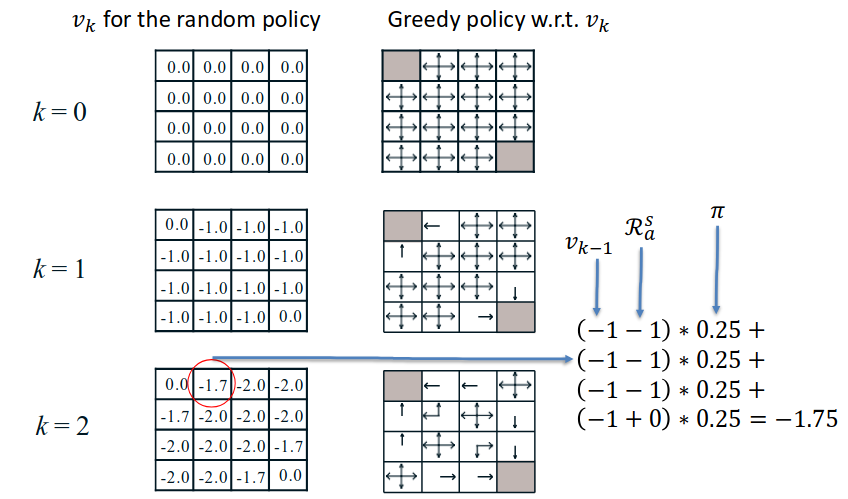
\includegraphics[width=0.9\textwidth]{images/L31.png}
    \caption{Example of prediction (left) and control (right). In the slides is showed that in the next time step the polict will remain the same, this means that the optimal polci has been reached. }
    \label{fig:student_markov_chain}
\end{figure}

\subsection{Policy Iteration}
\begin{wrapfigure}{r}{0.25\textwidth}
    \centering
    \vspace{-10pt}
    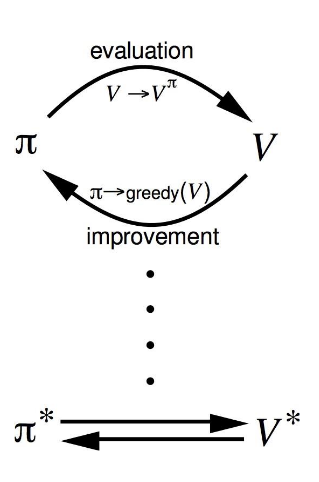
\includegraphics[width=\linewidth]{images/L32.png}
    \label{fig:TDlambda}
    \vspace{-10pt}
\end{wrapfigure}
La \emph{Policy Iteration} è il metodo di Dynamic Programming utilizzato per migliorare progressivamente una policy fino a ottenere una policy ottimale. L’idea di base consiste nell’alternare sistematicamente due fasi distinte: la valutazione della policy corrente e il suo miglioramento.

Il processo parte da una policy iniziale arbitraria $\pi$. Nella fase di \emph{policy evaluation}, la policy $\pi$ viene valutata calcolando la corrispondente value function $v^\pi$. Questa funzione rappresenta il return atteso partendo da ciascuno stato e seguendo sempre la policy $\pi$, ed è definita come:
\[
v^\pi(s) = \mathbb{E}_\pi \left[ R_{t+1} + \gamma R_{t+2} + \gamma^2 R_{t+3} + \dots \mid S_t = s \right]
\]
In pratica, $v^\pi$ viene stimata mediante l’Iterative Policy Evaluation, applicando ripetutamente la Bellman expectation equation fino alla convergenza.

Una volta ottenuta una stima accurata di $v^\pi$, si passa alla fase di \emph{policy improvement}. In questa fase, la policy viene aggiornata scegliendo, in ogni stato, l’azione che massimizza il valore atteso assumendo come riferimento la value function appena calcolata. La nuova policy $\pi'$ è definita come una policy greedy rispetto a $v^\pi$:
\[
\pi'(s) = \arg\max_{a \in \mathcal{A}} \sum_{s' \in \mathcal{S}} P_{ss'}^a \left[ R_s^a + \gamma v^\pi(s') \right]
\]
\begin{wrapfigure}{r}{0.3\textwidth}
    \centering
    \vspace{-10pt}
    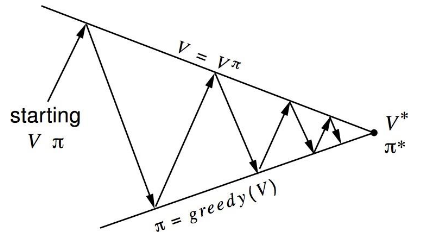
\includegraphics[width=\linewidth]{images/L33.png}
    \label{fig:TDlambda}
    \vspace{-10pt}
\end{wrapfigure}
Questo passo garantisce che la nuova policy $\pi'$ sia almeno altrettanto buona della policy precedente, cioè $\pi' \ge \pi$ per ogni stato.

In alcuni problemi semplici, come il classico Small Gridworld, una singola iterazione di policy improvement è sufficiente a ottenere direttamente la policy ottimale, ovvero si ha $\pi' = \pi^*$. In generale, tuttavia, è necessario ripetere più volte le due fasi di valutazione e miglioramento. Questo processo iterativo continua alternando policy evaluation e policy improvement fino a quando la policy non cambia più.

Un risultato fondamentale della Dynamic Programming è che la Policy Iteration, assumendo una conoscenza completa dell’MDP e uno spazio degli stati e delle azioni finito, converge sempre alla policy ottimale $\pi^*$. Questo rende la Policy Iteration uno degli algoritmi di riferimento per il problema di control nei Markov Decision Processes.

\subsection{Policy Improvement}

La \emph{Policy Improvement} è il passo che consente di migliorare una policy a partire dalla sua value function. Si consideri una policy deterministica $\pi$, tale che a ogni stato $s$ venga associata un’azione $a = \pi(s)$. Supponendo di conoscere la value function $v^\pi$, è possibile definire la corrispondente action-value function $q^\pi(s,a)$, che rappresenta il return atteso partendo dallo stato $s$, eseguendo l’azione $a$ e seguendo successivamente la policy $\pi$.

L’idea fondamentale del policy improvement consiste nel costruire una nuova policy $\pi'$ che, in ogni stato, selezioni in modo greedy l’azione che massimizza $q^\pi$. Formalmente, la policy migliorata è definita come:
\[
\pi'(s) = \arg\max_{a \in \mathcal{A}} q^\pi(s,a)
\]

Questa scelta garantisce un miglioramento locale del valore, poiché per ogni stato $s$ vale:
\[
q^\pi\bigl(s,\pi'(s)\bigr)
= \max_{a \in \mathcal{A}} q^\pi(s,a)
\ge q^\pi\bigl(s,\pi(s)\bigr)
= v^\pi(s)
\]

A partire da questa osservazione, è possibile dimostrare che la nuova policy $\pi'$ migliora la value function per tutti gli stati. In particolare:

\[
v^\pi(s)
\;\le\;
q^\pi\bigl(s,\pi'(s)\bigr)
\;=\;
\mathbb{E}_{\pi'} \left[ R_{t+1} + \gamma v^\pi(S_{t+1}) \mid S_t = s \right]
\;\le\;
\mathbb{E}_{\pi'} \left[ R_{t+1} + \gamma q^\pi\bigl(S_{t+1},\pi'(S_{t+1})\bigr) \mid S_t = s \right]
\]
\[
\le
\mathbb{E}_{\pi'} \left[ R_{t+1} + \gamma R_{t+2} + \gamma^2 q^\pi\bigl(S_{t+2},\pi'(S_{t+2})\bigr) \mid S_t = s \right]
\]
\[
\le\;
\mathbb{E}_{\pi'} \left[ R_{t+1} + \gamma R_{t+2} + \gamma^2 R_{t+3} + \dots \mid S_t = s \right]
=
v^{\pi'}(s)
\]

Da questa catena segue che:
\[
v^{\pi'}(s) \ge v^\pi(s) \qquad \forall s \in \mathcal{S}
\]
ovvero la policy $\pi'$ è almeno altrettanto buona della policy $\pi$ in tutti gli stati.

Se il processo di miglioramento non produce ulteriori cambiamenti, allora per ogni stato $s$ vale:
\[
q^\pi\bigl(s,\pi'(s)\bigr)
=
\max_{a \in \mathcal{A}} q^\pi(s,a)
=
q^\pi\bigl(s,\pi(s)\bigr)
=
v^\pi(s)
\]

In questo caso, la value function soddisfa l’equazione di Bellman di ottimalità:
\[
v^\pi(s) = \max_{a \in \mathcal{A}} q^\pi(s,a)
\]

Di conseguenza:
\[
v^\pi(s) = v^*(s) \qquad \forall s \in \mathcal{S}
\]
e quindi la policy $\pi$ è una policy ottimale.

\section{Modified Policy Iteration e Generalized Policy Iteration}

Nella Policy Iteration classica, ad ogni passo si eseguono due fasi distinte: si valuta la policy corrente $\pi$ fino a convergenza ottenendo $v^\pi$, e poi si migliora la policy rendendola greedy rispetto a $v^\pi$. In pratica, però, non è sempre necessario portare la policy evaluation fino alla convergenza esatta.

L’idea della \emph{Modified Policy Iteration} è proprio quella di \emph{interrompere prima} la policy evaluation. Invece di calcolare $v^\pi$ con accuratezza arbitraria, si può:
\begin{compactitemize}
    \item fermare l’Iterative Policy Evaluation quando la value function cambia meno di una certa soglia $\varepsilon$ (criterio di $\varepsilon$-convergenza),
    \item oppure semplicemente eseguire un numero fisso di iterazioni $k$ di policy evaluation e poi passare subito al policy improvement.
\end{compactitemize}

In altre parole, si alternano passi di valutazione \emph{parziale} della policy con passi di miglioramento greedy. Nel caso estremo in cui ci si fermi dopo una sola iterazione di policy evaluation ($k = 1$), la policy viene aggiornata ad ogni singola iterazione: questo caso limite risulta strettamente collegato alla \textbf{Value Iteration}.

Questa visione più generale del processo prende il nome di \textbf{Generalized Policy Iteration} (GPI). In GPI, qualunque algoritmo di policy evaluation (anche approssimato o tronco) può essere combinato con qualunque schema di policy improvement (ad esempio improvement greedy o $\varepsilon$-greedy). L’idea di fondo è che valutazione e miglioramento vengano portati avanti insieme, influenzandosi a vicenda, fino alla convergenza verso una policy ottimale.


\subsection{Principle of Optimality}

Il \emph{principle of optimality} formalizza una proprietà chiave delle policy ottimali nei Markov Decision Processes. Intuitivamente, afferma che una policy è ottimale se, oltre a essere ottimale a partire dallo stato iniziale, \emph{continua ad essere ottimale da ogni stato raggiungibile}.

Più precisamente, il teorema dice che una policy $\pi$ soddisfa
\[
v^\pi(s) = v^*(s)
\]
per uno stato $s$ se e solo se, per ogni stato $s'$ raggiungibile da $s$, la stessa policy è ottimale anche in $s'$, ossia
\[
v^\pi(s') = v^*(s') \quad \text{per tutti gli stati } s' \text{ raggiungibili da } s.
\]

Un modo equivalente di interpretarlo è: una policy ottimale può essere vista come composta da due parti: una \emph{prima azione ottimale} $A^*$ nello stato corrente, seguita da una policy che è a sua volta ottimale a partire dallo stato successore $S'$. Questo giustifica l’uso di equazioni ricorsive come la Bellman optimality equation: se conosciamo la soluzione dei “sottoproblemi” (gli stati successivi), possiamo ricostruire la soluzione dallo stato corrente.


\subsection{Deterministic Value Iteration}

La Deterministic Value Iteration è un metodo di Dynamic Programming utilizzato per calcolare direttamente la value function ottimale $v^*$ assumendo una conoscenza completa del modello dell’MDP. L’idea centrale è che, se fossero già noti i valori ottimali degli stati successivi $v^*(s')$, allora il valore ottimale di uno stato $s$ potrebbe essere calcolato immediatamente effettuando un one-step lookahead.

Questo principio è formalizzato dalla Bellman optimality equation, che nella Value Iteration viene utilizzata come regola di aggiornamento iterativo:
\[
v^*(s) \leftarrow \max_{a \in \mathcal{A}} \left( R_s^a + \gamma \sum_{s' \in \mathcal{S}} P_{ss'}^a \, v^*(s') \right)
\]

Questa equazione esprime il seguente meccanismo: per ogni stato $s$, si considerano tutte le azioni disponibili e, per ciascuna azione, si valuta il reward immediato atteso sommato al valore scontato degli stati successivi. Tra tutte le azioni, viene scelta quella che massimizza questo valore atteso. Il risultato rappresenta il miglior valore ottenibile partendo da $s$ e agendo in modo ottimale.

Poiché inizialmente i valori ottimali $v^*(s)$ non sono noti, la Value Iteration applica ripetutamente questo aggiornamento partendo da una stima iniziale arbitraria della value function. A ogni iterazione, i valori vengono raffinati utilizzando le stime precedenti, facendo dipendere il valore di uno stato dai valori degli stati successivi. In questo modo, l’informazione sui reward finali viene progressivamente propagata all’indietro nello spazio degli stati.

L’intuizione è quella di iniziare dagli stati terminali, o dagli stati con reward noti, e lavorare a ritroso verso tutti gli altri stati. Anche in presenza di cicli e di dinamiche stocastiche, il processo converge grazie all’uso del valore atteso sulle transizioni e al fattore di sconto $\gamma$, che garantisce la stabilità dell’aggiornamento. Una volta che la value function è conversa , la policy ottimale può essere ottenuta scegliendo, in ogni stato, l’azione greedy rispetto alla value function ottimale.


Nonostante il nome “deterministic value iteration” nei lucidi, l’algoritmo funziona perfettamente anche in MDP con transizioni stocastiche e con strutture con cicli (\emph{loopy MDP}), poiché le probabilità di transizione $P_{ss'}^a$ sono già incorporate nel calcolo dell’aspettativa. In sintesi, la Value Iteration aggiorna iterativamente i valori degli stati tramite la Bellman optimality equation finché la value function non si stabilizza; da questa, si estrae poi la policy ottimale come policy greedy rispetto a $v^*$.
\begin{figure}[H]
    \centering
    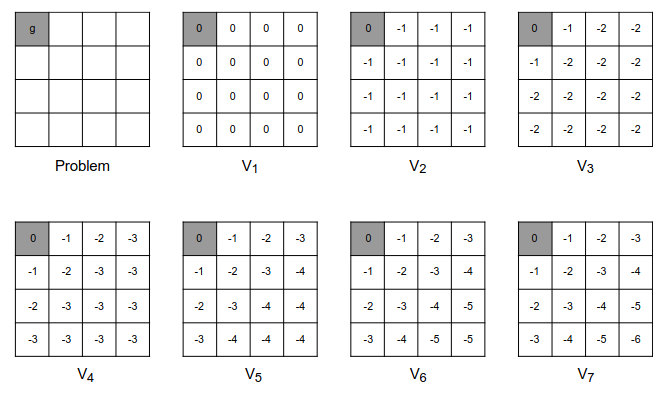
\includegraphics[width=0.9\textwidth]{images/L34.png}
    \caption{Example of backward value iteration }
    \label{fig:student_markov_chain}
\end{figure}

\subsection{Value Iteration: Control}

Il problema di control consiste nel determinare una policy ottimale $\pi^*$ partendo da una descrizione completa della dinamica dell’ambiente, ovvero dal modello dell’MDP. L’obiettivo è ottenere una policy che massimizzi il return atteso da ogni stato.

La Value Iteration risolve questo problema applicando iterativamente la Bellman optimality equation direttamente alla state-value function. A differenza della Policy Iteration, non viene mai mantenuta o valutata esplicitamente una policy durante il processo. L’algoritmo opera esclusivamente sui valori degli stati, aggiornandoli progressivamente fino alla convergenza verso la value function ottimale $v^*$.

L’aggiornamento fondamentale della Value Iteration è:
\[
v_{k+1}(s) = \max_{a \in \mathcal{A}} \left( R_s^a + \gamma \sum_{s' \in \mathcal{S}} P_{ss'}^a \, v_k(s') \right)
\]

A ogni iterazione $k+1$, per tutti gli stati $s \in \mathcal{S}$, il nuovo valore viene calcolato utilizzando esclusivamente i valori della precedente iterazione $v_k$. Questo aggiornamento è detto \emph{synchronous backup}, poiché tutti gli stati vengono aggiornati in parallelo a partire dalla stessa stima precedente.

La sequenza di value function $v_1 \rightarrow v_2 \rightarrow \dots$ converge progressivamente verso $v^*$, il fixed point della Bellman optimality equation. Durante questo processo non esiste una policy esplicita: le value function intermedie potrebbero non corrispondere ad alcuna policy reale. Solo una volta che la value function ha raggiunto la convergenza è possibile derivare una policy ottimale scegliendo, in ogni stato, l’azione greedy rispetto a $v^*$.

In sintesi, la Value Iteration può essere vista come la Bellman optimality equation trasformata in una regola di aggiornamento iterativa che consente di risolvere direttamente il problema di control.


\subsection{Synchronous Dynamic Programming Algorithms}

Gli algoritmi di Dynamic Programming sincroni condividono una struttura comune basata su aggiornamenti iterativi della value function. La distinzione principale tra i diversi algoritmi deriva dal tipo di equazione di Bellman utilizzata e dall’obiettivo del problema, che può essere di prediction o di control.

Nel caso della prediction, l’obiettivo è stimare la value function $v^\pi$ associata a una policy fissata. In questo scenario viene utilizzata la Bellman expectation equation e l’algoritmo risultante è l’Iterative Policy Evaluation.

Nel caso del control, l’obiettivo è calcolare la value function ottimale $v^*$. Questo può essere ottenuto in due modi diversi. Utilizzando la Bellman expectation equation insieme a un passo esplicito di policy improvement si ottiene la Policy Iteration, che alterna valutazione e miglioramento della policy. Utilizzando invece direttamente la Bellman optimality equation si ottiene la Value Iteration, che incorpora il miglioramento della policy nell’aggiornamento dei valori.

Tutti questi algoritmi operano tipicamente sulla state-value function. La complessità computazionale per ogni iterazione è dell’ordine di $O(mn^2)$, dove $n$ è il numero di stati e $m$ il numero di azioni. È possibile applicare concetti analoghi anche alla action-value function, ma in questo caso la complessità per iterazione cresce fino a $O(m^2 n^2)$, poiché è necessario considerare esplicitamente sia stati che coppie stato–azione.

Questa struttura sincrona, in cui tutti gli stati vengono aggiornati simultaneamente a ogni iterazione, rende gli algoritmi di Dynamic Programming concettualmente semplici e garantisce la convergenza, a patto di disporre di una conoscenza completa del modello dell’ambiente.
\begin{figure}[H]
    \centering
    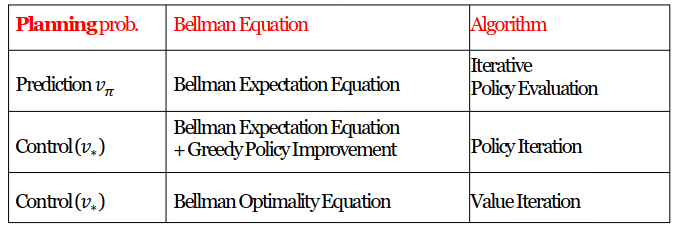
\includegraphics[width=0.9\textwidth]{images/F35.png}
    \label{fig:student_markov_chain}
\end{figure}

\section{Asynchronous Dynamic Programming}

Tutti i metodi di Dynamic Programming descritti finora utilizzano aggiornamenti sincroni (\emph{synchronous backups}), nei quali i valori di tutti gli stati vengono aggiornati in parallelo utilizzando la stessa stima precedente della value function. Questo approccio è concettualmente semplice, ma può risultare computazionalmente costoso quando il numero di stati è elevato.

L’Asynchronous Dynamic Programming introduce una strategia alternativa in cui gli stati vengono aggiornati individualmente, uno alla volta, e in un ordine arbitrario. A ogni passo, viene selezionato un singolo stato e su di esso viene applicato l’aggiornamento di Bellman appropriato, utilizzando immediatamente i valori più recenti disponibili. In questo modo, gli aggiornamenti non avvengono più in parallelo, ma in modo incrementale.

Questo approccio può ridurre significativamente il costo computazionale, poiché non è necessario aggiornare tutti gli stati a ogni iterazione. Inoltre, permette di concentrare il calcolo sugli stati più rilevanti o più frequentemente visitati. Nonostante la mancanza di sincronizzazione, è garantito che gli algoritmi asincroni convergano alla soluzione corretta, a patto che tutti gli stati continuino a essere selezionati e aggiornati nel tempo.

Esistono diversi criteri per scegliere quale stato aggiornare a ogni passo. Uno dei più semplici e fondamentali è il seguente.

\begin{compactitemize}
    \item \textbf{In-place Dynamic Programming}
    \item \textbf{Prioritized sweeping}
    \item \textbf{Real-Time dynamic programming}
\end{compactitemize}

\subsection{In-Place Dynamic Programming}

Nella Value Iteration sincrona classica, l’algoritmo mantiene due copie distinte della value function: una versione precedente $v_{\text{old}}$ e una versione aggiornata $v_{\text{new}}$. A ogni iterazione, per tutti gli stati $s \in \mathcal{S}$, il nuovo valore viene calcolato utilizzando esclusivamente $v_{\text{old}}$ secondo:
\[
v_{\text{new}}(s) \leftarrow \max_{a \in \mathcal{A}} \left( R_s^a + \gamma \sum_{s' \in \mathcal{S}} P_{ss'}^a \, v_{\text{old}}(s') \right)
\]
Al termine dell’aggiornamento di tutti gli stati, la copia vecchia viene sostituita con la nuova:
\[
v_{\text{old}}(s) \leftarrow v_{\text{new}}(s) \qquad \forall s \in \mathcal{S}
\]
Questo schema garantisce che tutti i backup utilizzino la stessa value function di riferimento, ma richiede di memorizzare due copie della value function e rallenta la propagazione dell’informazione, perché i nuovi valori non vengono sfruttati finché l’intera iterazione non è terminata.

Nell’In-Place Dynamic Programming, invece, si utilizza una sola copia della value function. Quando uno stato $s$ viene aggiornato, il suo valore viene immediatamente sovrascritto e reso disponibile per gli aggiornamenti successivi. L’aggiornamento assume la forma:
\[
v(s) \leftarrow \max_{a \in \mathcal{A}} \left( R_s^a + \gamma \sum_{s' \in \mathcal{S}} P_{ss'}^a \, v(s') \right)
\]
In questo modo, se uno stato successore $s'$ è già stato aggiornato nella stessa passata, il nuovo valore di $v(s')$ viene immediatamente utilizzato; se non lo è, viene utilizzato il valore precedente. Questo schema accelera la propagazione dell’informazione nello spazio degli stati ed è concettualmente analogo al metodo di Gauss--Seidel per la risoluzione di sistemi lineari. Pur introducendo una dipendenza dall’ordine di aggiornamento, l’In-Place Dynamic Programming garantisce comunque la convergenza alla value function corretta, a condizione che tutti gli stati vengano aggiornati ripetutamente.



\subsection{Prioritized Sweeping}

Il Prioritized Sweeping è una strategia di Asynchronous Dynamic Programming che affronta esplicitamente il problema di decidere quali stati aggiornare per primi e in quale ordine. L’idea di base è concentrare il calcolo sugli stati per i quali l’aggiornamento potrebbe produrre il maggiore cambiamento nella value function.

Per ogni stato $s$ viene calcolato il \emph{Bellman error}, definito come:
\[
\left| \max_{a \in \mathcal{A}} \left( R_s^a + \gamma \sum_{s' \in \mathcal{S}} P_{ss'}^a \, v(s') \right) - v(s) \right|
\]

Questo valore misura quanto l’attuale stima di $v(s)$ sia incoerente con la Bellman optimality equation. L’algoritmo seleziona quindi per l’aggiornamento lo stato con il Bellman error più grande, poiché è quello per cui l’update è potenzialmente più informativo.

Dopo aver aggiornato uno stato, anche gli stati che possono transire verso di esso (i cosiddetti predecessori) devono essere rivalutati, poiché il loro valore potrebbe dipendere dal nuovo valore appena calcolato. Questo richiede la conoscenza delle dinamiche inverse dell’ambiente. Dal punto di vista implementativo, il Prioritized Sweeping può essere realizzato in modo efficiente utilizzando una coda di priorità che ordina gli stati in base al loro Bellman error.


\subsection{Real-Time Dynamic Programming}

Il Real-Time Dynamic Programming (RTDP) combina i principi della Dynamic Programming con l’esperienza diretta di un agente che interagisce con l’ambiente. A differenza degli altri metodi, non viene considerato l’intero spazio degli stati, ma solo quelli effettivamente rilevanti per l’agente.

L’algoritmo prevede che un agente esegua episodi nell’ambiente seguendo una policy (tipicamente greedy rispetto alla value function corrente). Dopo ogni time-step, una volta osservati lo stato $S_t$, l’azione $A_t$ e il reward $R_{t+1}$, viene aggiornato esclusivamente il valore dello stato corrente $S_t$ secondo:
\[
v(S_t) \leftarrow \max_{a \in \mathcal{A}} \left( R_{S_t}^a + \gamma \sum_{s' \in \mathcal{S}} P_{S_t s'}^a \, v(s') \right)
\]

In questo modo, solo gli stati visitati dall’agente vengono aggiornati, evitando di sprecare calcolo su stati che non sono rilevanti per il comportamento reale. Il RTDP può essere visto come una forma di Dynamic Programming focalizzata online, che utilizza il modello dell’ambiente ma restringe gli aggiornamenti allo spazio di stati effettivamente esplorato. Se l’agente continua a visitare ripetutamente tutti gli stati rilevanti, il metodo converge alla value function ottimale.

\section{Full-Width Backups}

I metodi di Dynamic Programming utilizzano \emph{full-width backups}, ovvero aggiornamenti in cui, per ogni stato selezionato, vengono considerati esplicitamente tutte le azioni disponibili e tutti gli stati successori. Sia nel caso di backup sincroni sia asincroni, l’aggiornamento di un singolo stato richiede l’uso completo del modello dell’MDP, includendo le probabilità di transizione e la reward function.

Questo approccio consente di calcolare aggiornamenti esatti e garantisce la convergenza agli obiettivi di prediction o control. Per questo motivo, la Dynamic Programming risulta efficace per problemi di dimensione media, anche con milioni di stati, purché il modello dell’ambiente sia noto e gestibile.

Tuttavia, nei problemi di grandi dimensioni, la Dynamic Programming è pesantemente limitata dalla cosiddetta \emph{Bellman’s curse of dimensionality}. Il numero di stati $n = |\mathcal{S}|$ cresce esponenzialmente con il numero di variabili di stato, rendendo rapidamente proibitivo il costo computazionale. In tali scenari, anche un singolo full-width backup può risultare troppo costoso, rendendo necessarie tecniche alternative basate su approssimazione, campionamento o apprendimento diretto dall’esperienza.


